\documentclass[12pt]{article}

\usepackage{geometry}                % See geometry.pdf to learn the layout options. There are lots.
\geometry{margin=5em}                   % ... or a4paper or a5paper or ... 
%\usepackage[parfill]{parskip}    % Activate to begin paragraphs with an empty line rather than an indent
\usepackage{latexsym,amsfonts,amsmath,amssymb,amsthm}
\usepackage{enumerate}
\usepackage{epstopdf}
\usepackage{color,graphicx, subfigure}
\usepackage[usenames,dvipsnames]{xcolor}
\usepackage{tikz}
\usepackage{gensymb}
\usepackage{hyperref}
\usetikzlibrary{calc,decorations.markings, positioning, fadings}
\usepackage{fancyhdr}
\usepackage{capt-of}

% Table spacing
\setlength{\tabcolsep}{6pt} % Default value: 6pt
\renewcommand{\arraystretch}{1.2} % Default value: 1

\newtheorem{Exercise}{Exercise}[section]
\newenvironment{exercise}{\begin{Exercise}\rm}{\end{Exercise}}

\newcommand{\widthtwofigures}{0.47\textwidth}
\newcommand{\widththreefigures}{0.32\textwidth}

\begin{document}
\title{\vspace{-2em}
Stretching and Shrinking}
\date{}
\maketitle
\vspace{-6em}
\thispagestyle{fancy}
\pagestyle{fancy}
\rhead{Tiago Salvador}
\lhead{Fall 2017} 
\chead{Math 115: Calculus I (Section 29 and 49)}
\pagenumbering{gobble}

\vspace{4ex}

Here we discuss stretching and shrinking. If $k > 1$, then the graph of $kf(x)$ is the graph of $f(x)$ stretched by a factor of $k$ in the vertical direction (since each $y$-value is multiplied by the same number $k$). On the other hand, when $0 < k < 1$, the graph of $kf(x)$ is the graph of $f(x)$ shrunk by a factor of $1/k$. See Figure~1 for an example with different values of $k$. Notice how the graph of $f(x)/3$ is three times vertically smaller than the graph of $f(x)$.

It is also possible to stretch and shrink a graph horizontally, although the effects can be rather counter intuitive and often lead to confusion. If $k > 1$, then the graph of $f(kx)$ is the graph of $f(x)$ shrunk by a factor of $k$ in the horizontal direction. Notice how this is the opposite of the vertical scaling. A good way to understand this is to think about the domain of $f(x)$ and $f(kx)$. Let us take a look at the example in Figure~2. The domain of $f(x)$ is $[-2,4]$ and so the domain of $f(2x)$ is $[-1,2]$ since
\[
-2 \leq 2x \leq 4 \Longleftrightarrow -1 \leq x \leq 2.
\]
The domain is $2$ times smaller, i.e., it shrunk by a factor of $2$. The tables below are also a good way to understand this.

On the other hand, if $0 < k < 1$, then the graph of $f(kx)$ is the graph of $f(x)$ stretched by a factor of $1/k$ in the horizontal direction. Again, let us look at the domains of the functions in Figure~2. The domain of $f(x)$ is $[-2,4]$ and so the domain of $f(x/2)$ is $[-4,8]$ since
\[
-2 \leq x/2 \leq 4 \Longleftrightarrow -4 \leq x \leq 8.
\]

\begin{figure}[htp]
\centering
\begin{minipage}[t]{\widthtwofigures}
\centering
\vspace{0pt}
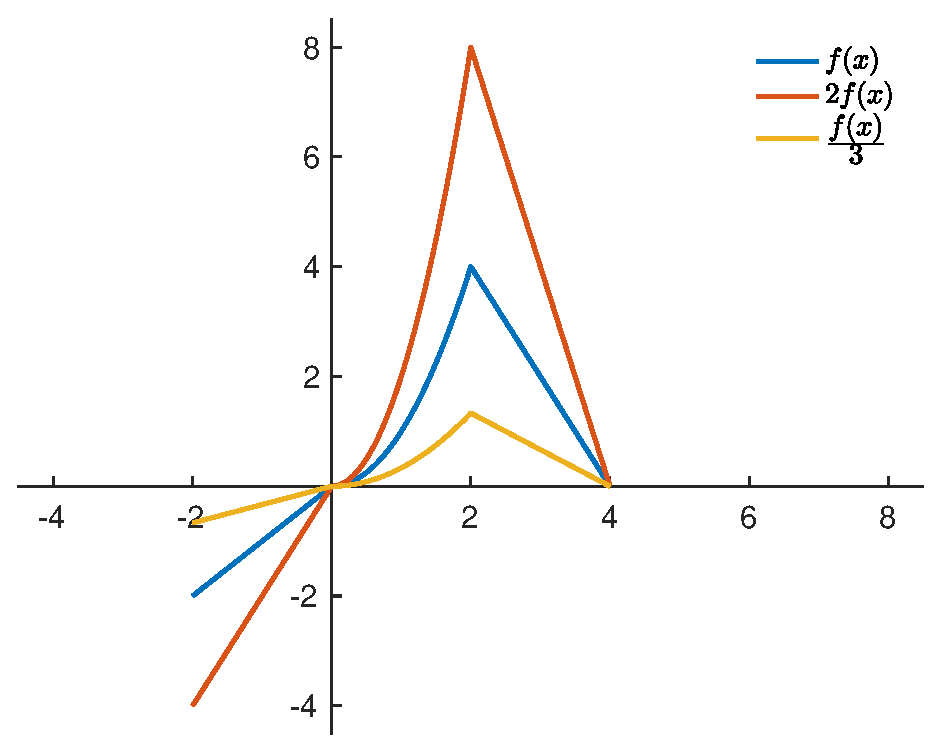
\includegraphics[width=\textwidth]{stretchshrinkvertical}
\caption{Plot of $f(x)$ and $kf(x)$ with $k = 2$ and $k = 1/3$.}
\end{minipage}\hfill
\begin{minipage}[t]{\widthtwofigures}
\centering
\vspace{0pt}
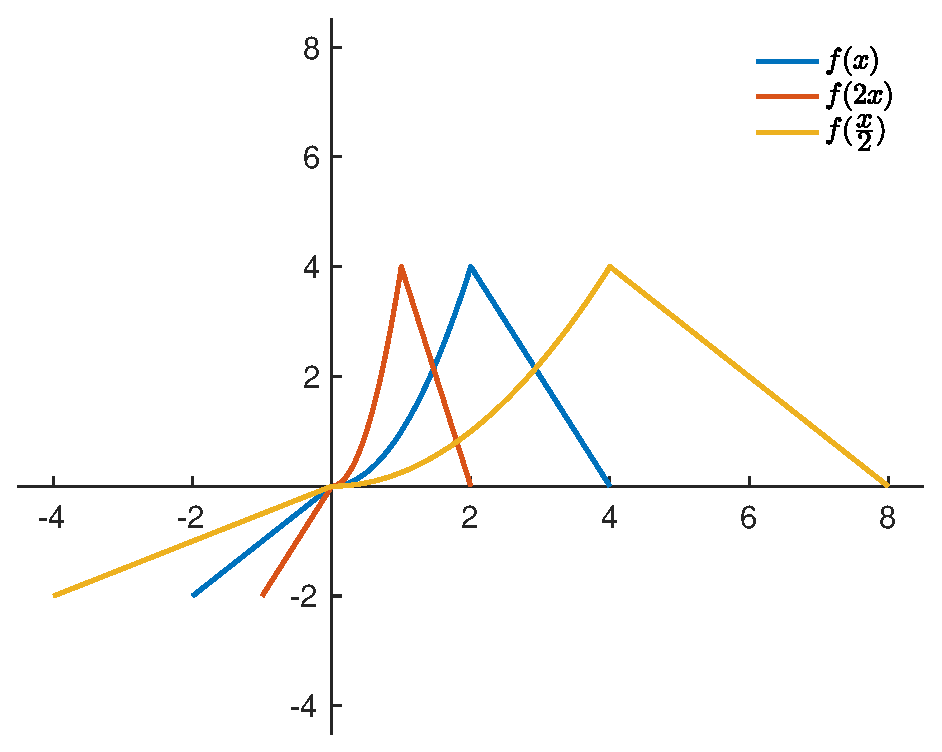
\includegraphics[width=\textwidth]{stretchshrinkhorizontal}
\caption{Plot of $f(x)$ and $f(kx)$ with $k = 1/2$ and $k = 2$.}
\end{minipage}
\end{figure}


\newpage

\begin{figure}[htp]
\centering
\begin{minipage}[t]{\widththreefigures}
\centering
\vspace{0pt}
\begin{tabular}{c|c}
$x$	& $f(x)$\\ \hline
-2	& -2\\ \hline
0	& 0	\\ \hline
2	& 4	\\ \hline
4	& 0	\\
\end{tabular}
\end{minipage}\hfill
\begin{minipage}[t]{\widththreefigures}
\centering
\vspace{0pt}
\begin{tabular}{c|c}
$x$	& $f(2x)$ \\ \hline
-1	& -2 \\ \hline
0	& 0	\\ \hline
1	& 4	\\ \hline
2	& 0	\\
\end{tabular}
\end{minipage}
\begin{minipage}[t]{\widththreefigures}
\centering
\vspace{0pt}
\begin{tabular}{c|c}
$x$	& $f(x/2)$ \\ \hline
-4	& -2 \\ \hline
0	& 0\\ \hline
4	& 4\\ \hline
8	& 0 \\
\end{tabular}
\end{minipage}
\end{figure}

In short, given a function $f(x)$ and a constant $k$,
\begin{itemize}
	\item if $k > 1$, $kf(x)$ stretches the graph of $f(x)$ vertically by a factor of $k$.
	\item if $0 < k < 1$, $kf(x)$ shrinks the graph of $f(x)$ vertically by a factor of $1/k$.
	\item if $k > 1$, $f(kx)$ shrinks the graph of $f(x)$ horizontally by a factor of $k$.
	\item if $0 < k < 1$, $kf(x)$ stretches the graph of $f(x)$ horizontally by a factor of $1/k$.
\end{itemize}

%\newpage
%
%\begin{figure}[htp]
%\centering
%\begin{minipage}[t]{\widthtwofigures}
%\centering
%\vspace{0pt}
%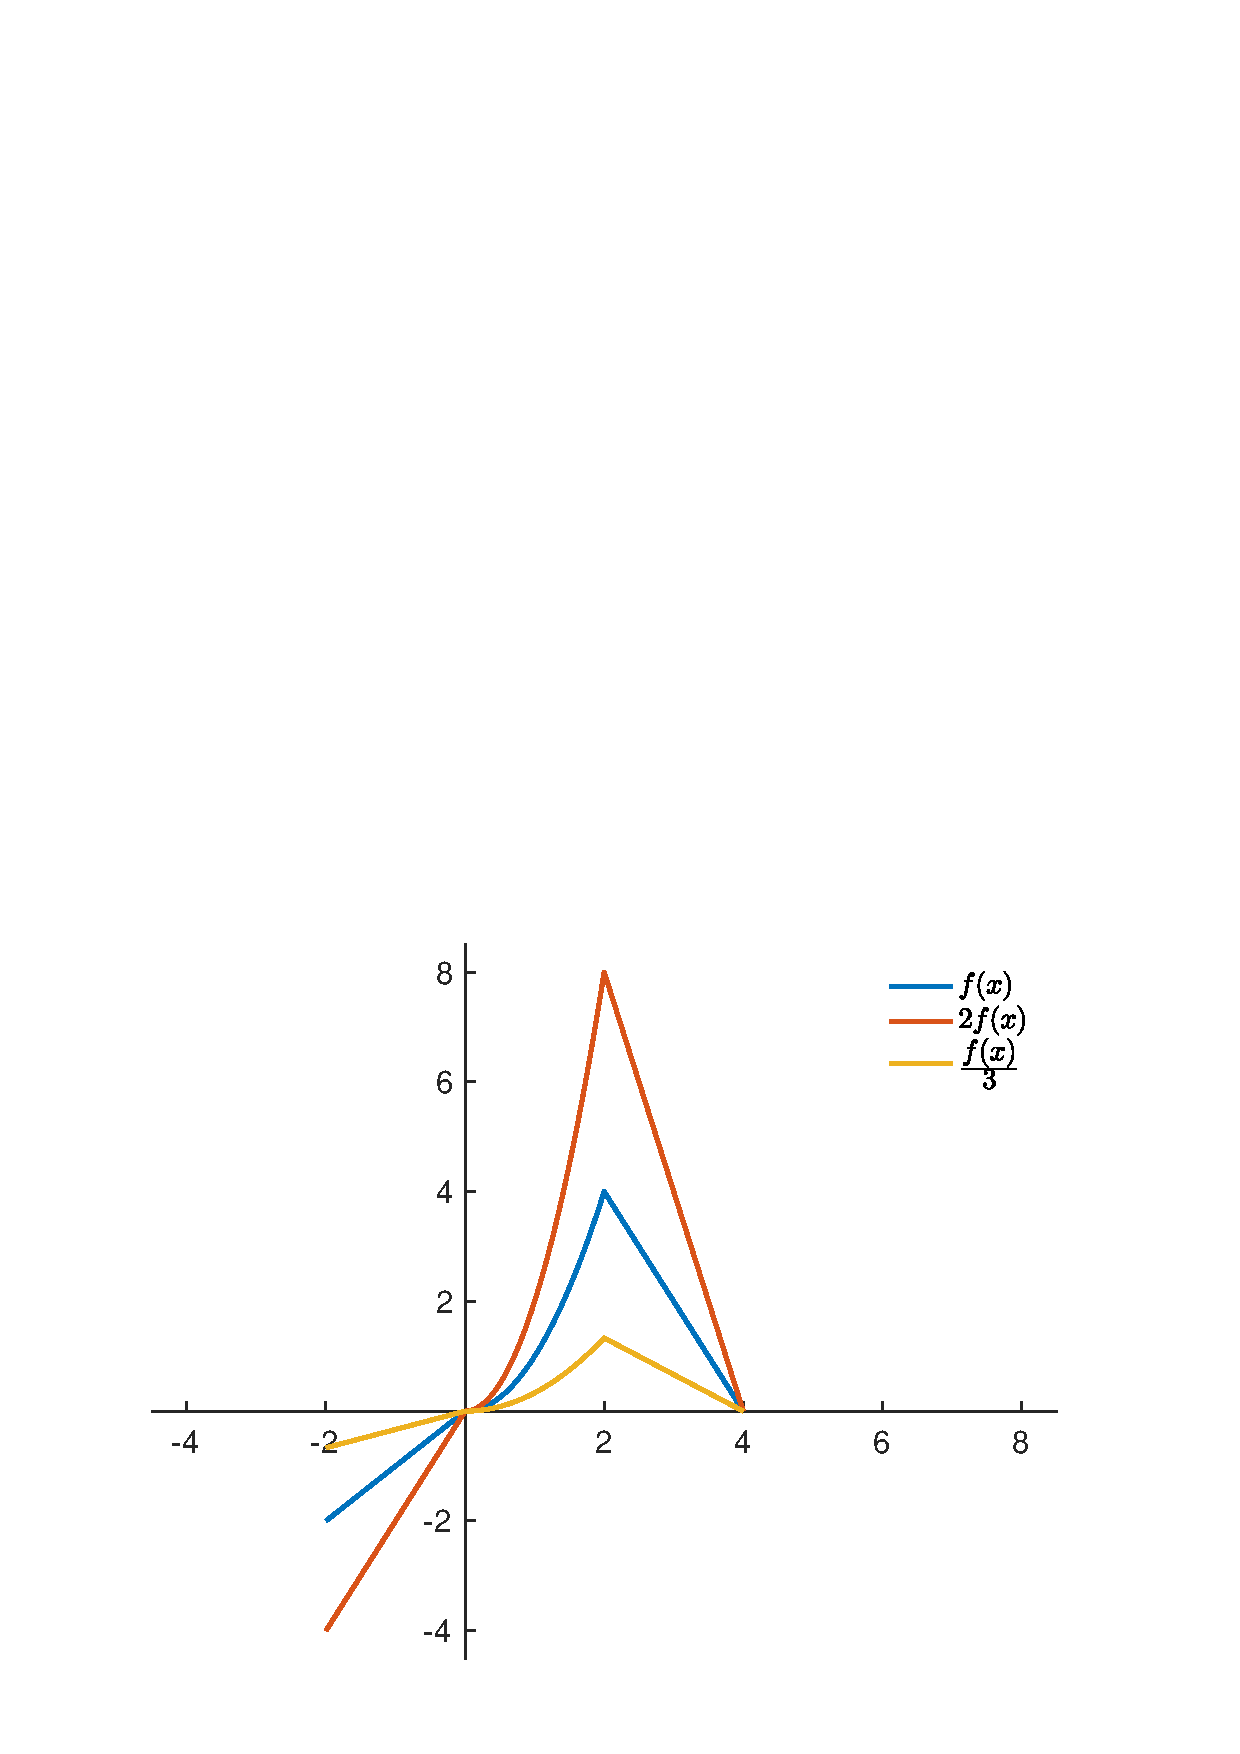
\includegraphics[width=\textwidth]{stretchshrinkvertical.pdf}
%\caption{Plot of $f(x)$ and $kf(x)$ with $k = 1/2$ and $k = 3$.}
%\end{minipage}\hfill
%\begin{minipage}[t]{\widthtwofigures}
%\centering
%\vspace{0pt}
%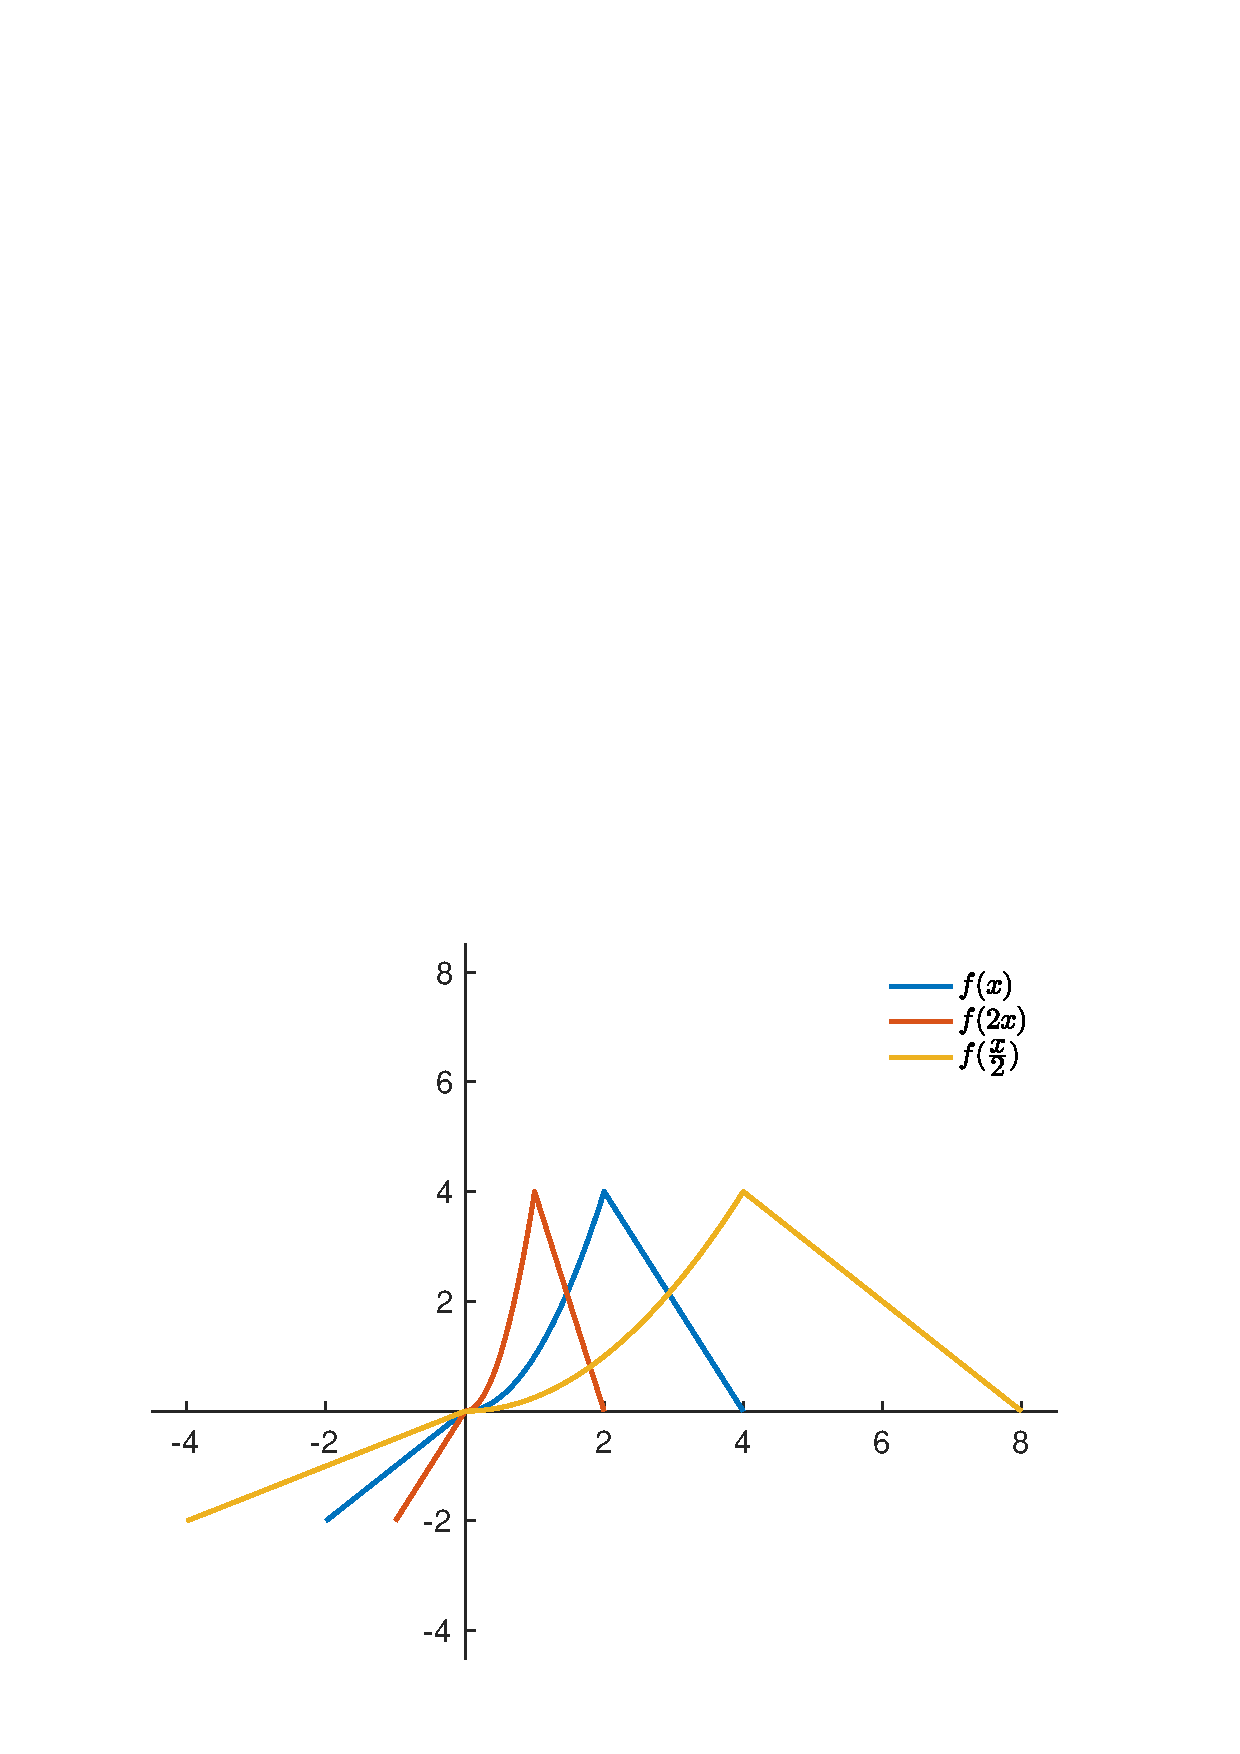
\includegraphics[width=\textwidth]{stretchshrinkhorizontal.pdf}
%\caption{Plot of $f(x)$ and $f(kx)$ with $k = 1/2$ and $k = 2$.}
%\end{minipage}
%\end{figure}
%
%Instead of multiplying the whole function by a constant, we can instead multiply the argument of the function by a positive constant. In this case, each $x$-value is stretched or shrunk by that multiple (again) depending on the magnitude of the constant. See Figure 2 for an example with different values of $k$. In general, given a function $f(x)$ and $k > 0$, $f(kx)$ shrinks  the graph horizontally if $k > 1$ or stretches the graph horizontally if $0 < k < 1$. Notice how this is the exact opposite of when we multiply the function by a constant. It is rather counter intuitive, so look at the tables below to convince yourself of this.
%
%
%we have the following
%
%The graph of a positive constant multiple of a given function is easy to visualize: each $y$-value is stretched or shrunk by that multiple depending on the magnitude of the constant. See Figure~1 for an example with different values of $k$. In general, we have the following: multiplying a function by a constant, $k$, stretches the graph vertically if $k > 1$ and shrinks the graph vertically if $0 < k < 1$.

\end{document}
